\documentclass[11pt,a4paper]{article}

\usepackage[T1]{fontenc}
\usepackage[utf8]{inputenc}
\usepackage{mathpazo}
\usepackage{courier}
\usepackage[margin=2.4cm]{geometry}
\usepackage{microtype}
\usepackage{amsmath,amssymb}
\usepackage{booktabs}
\usepackage{tabularx}
\usepackage{xcolor}
\usepackage{tikz}
\usetikzlibrary{arrows.meta,positioning,fit}
\usepackage{pgfplots}
\pgfplotsset{compat=1.18}
\usepackage{listings}
\usepackage{caption}
\usepackage[hidelinks]{hyperref}
\usepackage{enumitem}
\setlist{nosep,leftmargin=1.4em}

\definecolor{seriesA}{HTML}{2A78D6}
\definecolor{seriesB}{HTML}{EB6834}
\definecolor{inkmuted}{HTML}{52514E}
\definecolor{boxfill}{HTML}{EEF2FA}

\lstset{basicstyle=\ttfamily\footnotesize,breaklines=true,columns=fullflexible,
  frame=single,rulecolor=\color{inkmuted!40},framesep=4pt,xleftmargin=4pt,xrightmargin=4pt,
  literate={é}{{\'e}}1 {É}{{\'E}}1 {è}{{\`e}}1 {à}{{\`a}}1 {ç}{{\c{c}}}1 {œ}{{\oe}}1 {ê}{{\^e}}1 {î}{{\^i}}1}

\newcommand{\code}[1]{\texttt{#1}}

\title{\textbf{RootCause-SLM}\\[2pt]
\large Detecting HDFS anomalies and explaining them with a small language model,\\ and measuring where the explanations fail}
\author{Yifan Wang\\ \small Télécom Paris\\ \small \url{https://github.com/NafiyTP/RootCause-SLM}}
\date{October 2026}

\begin{document}
\maketitle

\begin{abstract}
Infrastructure logs are often too sensitive to send to an external API, which makes small
language models that run locally attractive for log analysis. RootCause-SLM is a two-stage
pipeline for HDFS logs. The first stage groups raw lines into block sessions and classifies
each block from counts of message templates; on the full HDFS\_v1 log (11.2M lines, 575k
blocks, chronological split) a logistic regression reaches an F1 of 0.973. The second stage
explains a flagged block with Qwen2.5-1.5B-Instruct fine-tuned with LoRA on explanations
written by Llama 3.3-70B. The student reproduces its teacher better than every baseline
(ROUGE-L 0.506 on the reasoning, against 0.456 for template retrieval) and, with batching,
costs about seven times less per explanation than calling the teacher. An audit against the
raw logs shows the limit of this setup: on 250 anomalous test lines, the explanation of the
fine-tuned model never mentions what is actually wrong with the block, and the teacher's
explanation does so once. The evidence (a write that never completed, a failed delete, an
orphan block) lies in other lines of the block, so the model can only guess, and distillation
copies the guess faithfully. A simple rule that lists the events missing from a flagged block
explains it better at no cost. On BGL, a less regular system, the same detector drops to
F1 0.676 and a log-level rule does better, because most test windows contain templates never
seen during training.
\end{abstract}

\section{Introduction}

Log anomaly detection on public benchmarks is largely a solved problem for regular systems
such as HDFS, where a block id ties every line to a session and a few dozen message types
describe almost every event~\cite{xu2009,he2016,du2017,zhu2023}. What operators actually need
after an alert is the next step: an explanation of what went wrong. Large language models
can write such explanations, but sending production logs to an external API is often not
allowed. This project asks how far a small model, small enough to run on a single cheap GPU,
can go on that task, and how to tell whether its explanations are right.

The project went through three versions. The first one only had the explanation model, with
the anomaly label given as input; the label had to come from somewhere, so the second
version added a block-level detector and a script that chains both. The third version added
what this report is mostly about: a benchmark of speed and cost, a test on a second system,
and an audit that checks the explanations against the raw logs instead of against the
teacher that produced the training data.

\paragraph{Contributions.}
\begin{itemize}
  \item A block-level detector evaluated on the full HDFS\_v1 log with a chronological split,
        compared with a log-level rule and PCA, and the same detectors on BGL.
  \item A teacher-student explanation model (Llama 3.3-70B $\rightarrow$ Qwen2.5-1.5B with LoRA),
        evaluated against five baselines, with its inference cost measured on a T4.
  \item An audit showing that neither the teacher nor the student identifies the block-level
        evidence, with an analysis of why, and a zero-cost alternative (missing events) that does.
\end{itemize}

\section{Data}

\paragraph{HDFS\_v1.} The Loghub release of the HDFS logs collected by Xu et al.\ from Hadoop
map-reduce jobs on more than 200 Amazon EC2 nodes in 2008~\cite{xu2009,zhu2023}: 11,175,629 lines and 575,061 blocks, of which
2.9\% are labelled anomalous by Hadoop experts. Labels are per block. A line belongs to every
block whose id (\code{blk\_-?\textbackslash d+}) it mentions.

\paragraph{BGL.} Logs of the Blue Gene/L supercomputer at Lawrence Livermore National
Laboratory~\cite{oliner2007}, 4,713,493 lines. There is no session id, and every line carries
its own label: \code{-} for normal, otherwise an alert category.

\paragraph{Explanation dataset.} For the explanation model, each line gets the label of its
block, and Llama 3.3-70B (through the Groq API) writes two fields in French: a short
\code{cause} and a three-step \code{raisonnement}. The teacher never decides the label. The
training set has 1,999 lines (1,930 normal, 69 anomalous, split 85/15 into train and
validation); the anomalous lines cover 29 different causes and the whole set only 15 message
templates. The test set has 527 lines (277 normal, 250 anomalous) taken from blocks that never
appear in training, with anomalies oversampled so that the metrics say something about them.

\section{Method}

\begin{figure}[t]
\centering
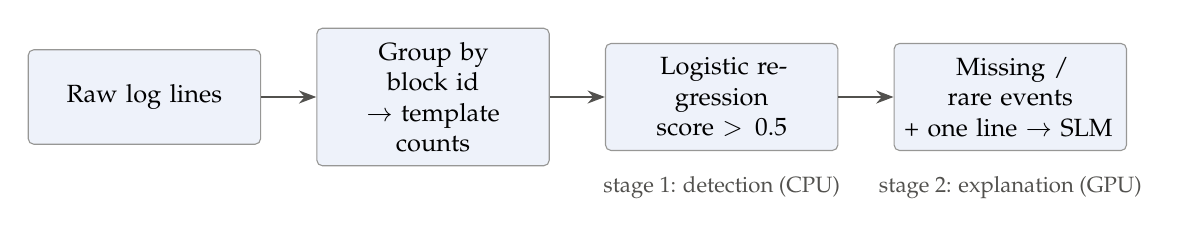
\begin{tikzpicture}[
  node distance=5mm and 7mm,
  box/.style={draw=inkmuted!60, fill=boxfill, rounded corners=2pt, align=center,
              font=\small, inner sep=5pt, minimum height=12mm, text width=26mm},
  arr/.style={-{Stealth[length=2.2mm]}, inkmuted, thick}]
  \node[box] (raw) {Raw log lines};
  \node[box, right=of raw] (grp) {Group by block id\\ $\rightarrow$ template counts};
  \node[box, right=of grp] (det) {Logistic regression\\ score $>0.5$};
  \node[box, right=of det] (exp) {Missing / rare events\\ + one line $\rightarrow$ SLM};
  \draw[arr] (raw) -- (grp);
  \draw[arr] (grp) -- (det);
  \draw[arr] (det) -- (exp);
  \node[font=\footnotesize, text=inkmuted, below=2mm of det] {stage 1: detection (CPU)};
  \node[font=\footnotesize, text=inkmuted, below=2mm of exp] {stage 2: explanation (GPU)};
\end{tikzpicture}
\caption{The pipeline. Detection runs on the whole block; the language model sees a single line.}
\label{fig:pipeline}
\end{figure}

\subsection{Templates}
Each line is reduced to a template: the date, time and process id are dropped, then block
ids, IP addresses (with an optional port), paths and remaining numbers are replaced by
\code{<BLK>}, \code{<IP>}, \code{<PATH>} and \code{<N>}, in that order. On HDFS this yields 54
templates over the training period. For BGL the masking also replaces hexadecimal values and
the message is prefixed with the component and the level. No learned parser such as
Drain~\cite{he2017drain} is used.

\subsection{Block-level detection}
A block becomes a vector $x \in \mathbb{N}^{V+1}$ of template counts, with one extra column
\code{<UNK>} that collects the templates absent from training (a new kind of message is
exactly what one wants to notice, so it is kept rather than dropped). Blocks are sorted by
their first line and split chronologically: the first 80\% for training, the last 20\% for
testing, so the model never sees the future. Three detectors are compared.
\begin{itemize}
  \item \textbf{Log-level rule}: a block is anomalous if one of its lines is not INFO
        (on BGL: FATAL, FAILURE, SEVERE or ERROR). This is what one does without learning.
  \item \textbf{PCA}~\cite{xu2009}: fit on standardised $\log(1+x)$, keep the components that
        explain 95\% of the variance, and score a block by its squared reconstruction error.
        The threshold is the 97th percentile of the training scores; no label is used.
  \item \textbf{Logistic regression} on $\log(1+x)$ with balanced class weights (anomalies are
        about 3\% of the blocks), threshold 0.5.
\end{itemize}
On BGL, a session is a 60-minute window over the whole machine, anomalous if it contains at
least one alert line.

\subsection{Explanation model}
The student is Qwen2.5-1.5B-Instruct~\cite{qwen2025}. The prompt is the ChatML system message
below, then the line (truncated to 300 characters) and its label; the target is the teacher's
JSON. The loss is computed only on the answer tokens (prompt positions set to $-100$).
LoRA~\cite{hu2022} adapters of rank 16 ($\alpha=32$, dropout 0.05) are trained on the four
attention projections, 4.36M parameters or 0.28\% of the model. Because anomalies are 3.5\%
of the training lines, a weighted random sampler draws both classes about equally often.
Training uses AdamW with learning rate $2\cdot10^{-4}$, 5\% linear warm-up then cosine decay,
an effective batch size of 16 and 5 epochs on a Colab T4 (Figure~\ref{fig:train}).

\begin{lstlisting}
Tu es un expert en systèmes distribués Hadoop/HDFS. Étant donné un log et son label
(Normal ou Anomaly), tu fournis une cause technique précise et un raisonnement en 3 étapes.
\end{lstlisting}

\begin{figure}[t]
\centering
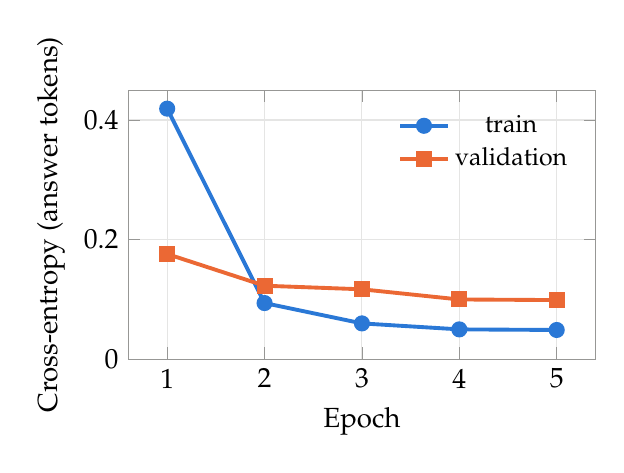
\begin{tikzpicture}
\begin{axis}[
  width=0.62\linewidth, height=5cm,
  xlabel={Epoch}, ylabel={Cross-entropy (answer tokens)},
  xtick={1,2,3,4,5}, ymin=0, ymax=0.45,
  grid=major, grid style={inkmuted!15},
  axis line style={inkmuted!60}, tick style={inkmuted!60},
  legend style={draw=none, fill=none, font=\small, at={(0.97,0.95)}, anchor=north east},
  every axis plot/.append style={line width=1.4pt, mark size=2.2pt}]
\addplot[color=seriesA, mark=*] coordinates {(1,0.419) (2,0.094) (3,0.060) (4,0.050) (5,0.049)};
\addlegendentry{train}
\addplot[color=seriesB, mark=square*] coordinates {(1,0.176) (2,0.123) (3,0.117) (4,0.100) (5,0.099)};
\addlegendentry{validation}
\end{axis}
\end{tikzpicture}
\caption{Training curves. Validation perplexity is already 1.19 after one epoch and ends at 1.10:
the targets are short and very repetitive.}
\label{fig:train}
\end{figure}

\subsection{From a flagged block to an explanation}
The model was trained on single lines, so the pipeline has to choose one. For every flagged
block it takes the line whose template pushes the score up the most: a template never seen in
training if there is one, otherwise the one with the largest coefficient. That line is sent
with the label \emph{Anomaly}. Independently of the model, the pipeline also lists the
\emph{missing events}: the templates that at least 90\% of the normal training blocks contain
but this block does not.

\section{Results}

\subsection{Detection on HDFS}

\begin{table}[t]
\centering
\caption{Detection on the full HDFS\_v1 log. Test set: the last 115,013 blocks (1.5\% anomalous).}
\label{tab:hdfs}
\begin{tabular}{lrrrr}
\toprule
Detector & Precision & Recall & F1 & Flagged \\
\midrule
WARN/ERROR rule & 1.000 & 0.248 & 0.398 & 417 \\
PCA (unsupervised) & 0.379 & 0.051 & 0.090 & 227 \\
Logistic regression & \textbf{0.955} & \textbf{0.992} & \textbf{0.973} & 1,744 \\
\bottomrule
\end{tabular}
\end{table}

Table~\ref{tab:hdfs} gives the results. The rule never raises a false alarm but finds only a
quarter of the anomalies: three quarters of the anomalous blocks contain only INFO lines. The
logistic regression finds almost all of them. Its largest weights go to the templates one
would expect: a redundant \code{addStoredBlock}, an \code{addStoredBlock} for a block that
belongs to no file, a failed delete (\emph{BlockInfo not found in volumeMap}) and a replication
time-out. Parsing, features and prediction together run at about 115k lines per second on one
CPU core.

PCA ranks the blocks well (ROC AUC 0.98 on the test set) but its threshold does not transfer:
it is fixed on the training period, where 3.3\% of the blocks are anomalous, against 1.5\% in
the test period, and the scores shift between the two. With the threshold fixed on training
scores it flags only 0.2\% of the test blocks. A usable threshold needs labels or a known
anomaly rate.

The detector also needs complete sessions. On an extract made of the first 104,815 lines, the
same logistic regression only reaches F1 0.27: the most recent test blocks are cut at the end
of the extract, look exactly like writes that never completed, and are flagged. On a stream,
a block has to be closed before it can be scored.

\subsection{Generalisation to BGL}

\begin{table}[t]
\centering
\caption{The same detectors on BGL, 60-minute windows. Test set: the last 724 windows (18.6\% anomalous).
13,603 templates in training; 412 test windows (57\%) contain at least one unseen template.}
\label{tab:bgl}
\begin{tabular}{lrrrr}
\toprule
Detector & Precision & Recall & F1 & Flagged \\
\midrule
Level rule (FATAL/FAILURE/SEVERE/ERROR) & 0.734 & \textbf{1.000} & \textbf{0.846} & 184 \\
PCA (unsupervised) & 0.203 & 0.541 & 0.295 & 359 \\
Logistic regression & \textbf{0.972} & 0.518 & 0.676 & 72 \\
\bottomrule
\end{tabular}
\end{table}

\begin{figure}[t]
\centering
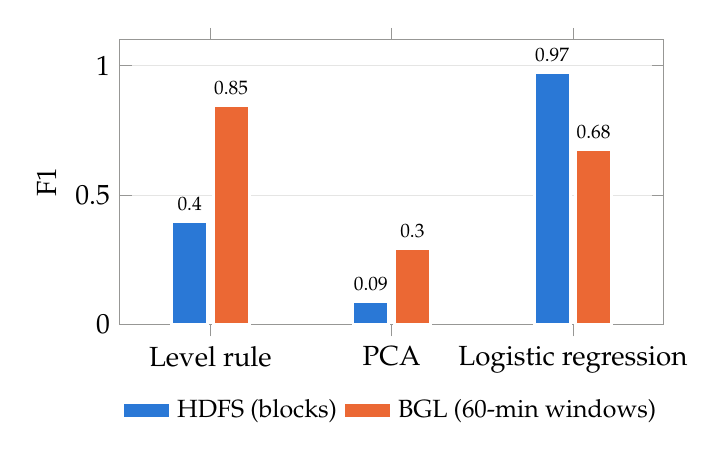
\begin{tikzpicture}
\begin{axis}[
  ybar, bar width=13pt, width=0.7\linewidth, height=5.2cm,
  ymin=0, ymax=1.1, ylabel={F1},
  symbolic x coords={Level rule, PCA, Logistic regression}, xtick=data,
  enlarge x limits=0.25,
  nodes near coords, nodes near coords style={font=\scriptsize, text=black},
  every node near coord/.append style={/pgf/number format/.cd, fixed, precision=2},
  ymajorgrids, grid style={inkmuted!15},
  axis line style={inkmuted!60}, tick style={inkmuted!60},
  legend style={draw=none, fill=none, font=\small, at={(0.5,-0.22)}, anchor=north, legend columns=2},
  area legend]
\addplot[fill=seriesA, draw=white, line width=1pt] coordinates {(Level rule,0.398) (PCA,0.090) (Logistic regression,0.973)};
\addlegendentry{HDFS (blocks)}
\addplot[fill=seriesB, draw=white, line width=1pt] coordinates {(Level rule,0.846) (PCA,0.295) (Logistic regression,0.676)};
\addlegendentry{BGL (60-min windows)}
\end{axis}
\end{tikzpicture}
\caption{F1 of each detector on the two systems. The ranking between the rule and the learned
model flips.}
\label{fig:f1}
\end{figure}

On BGL the ranking flips (Table~\ref{tab:bgl}, Figure~\ref{fig:f1}). The logistic regression is
still very precise but misses half of the anomalous windows, and the level rule wins. The
template counts explain it: the masking written for HDFS leaves 13,603 templates on BGL, and
57\% of the test windows contain at least one template never seen in training. All of them
land in the single \code{<UNK>} column, so a new kind of failure looks almost like a new kind
of normal message. Counting templates only works when templates are stable; on a less regular
system it needs a real parser and a model that can place unseen templates.

\subsection{Explanations compared with the teacher}

\begin{table}[t]
\centering
\caption{Explanation quality on the 527 test lines, measured against the teacher's annotations.
Greedy decoding; the fine-tuned model gets exactly its training prompt.}
\label{tab:expl}
\small\setlength{\tabcolsep}{4pt}
\begin{tabular}{lrrrrr}
\toprule
 & Valid & Cause & \multicolumn{2}{c}{ROUGE-L} & BERTScore \\
System & JSON & exact & cause & reasoning & reasoning \\
\midrule
Most frequent cause & 100\% & 0.461 & 0.594 & 0.347 & 0.797 \\
Majority cause per label & 100\% & 0.461 & 0.589 & 0.356 & 0.783 \\
Template retrieval & 100\% & 0.548 & 0.860 & 0.456 & 0.825 \\
Qwen2.5-1.5B zero-shot & 6.5\% & 0.000 & 0.008 & 0.017 & 0.048 \\
Qwen2.5-1.5B few-shot (3 ex.) & 100\% & 0.000 & 0.393 & 0.292 & 0.778 \\
Qwen2.5-1.5B + LoRA & \textbf{100\%} & \textbf{0.617} & \textbf{0.874} & \textbf{0.506} & \textbf{0.836} \\
\bottomrule
\end{tabular}
\end{table}

Table~\ref{tab:expl} compares the fine-tuned model with three non-neural baselines and with
the base model prompted zero-shot and few-shot. ROUGE-L~\cite{lin2004} and
BERTScore~\cite{zhang2020} are computed against the teacher. Template retrieval, which copies
the annotation of a training line with the same template and label, is the baseline that
matters. The fine-tuned model beats it by 0.050 ROUGE-L on the reasoning (paired bootstrap
95\% CI $[0.038, 0.064]$) and doubles the exact cause match on anomalies (0.284 against 0.140);
on the reasoning of anomalous lines the two are tied (0.455 against 0.461). Zero-shot, the base
model mostly fails on format (code fences, broken strings, running out of tokens); three
examples fix the format, but it then paraphrases the causes. So, measured against its teacher,
the distillation works.

\subsection{Audit: do the explanations find the real cause?}

The scores above say how close each system gets to the teacher, not whether the cause is
right. To check that, the full block of every anomalous test line was rebuilt from
\code{HDFS.log} and its block-level evidence extracted with the detector's statistics: if
the events that normal blocks end with (including the \code{addStoredBlock} that confirms a
replica was stored) are missing, the write never completed; otherwise the rare events it
contains (seen in fewer than 5\% of normal blocks) name the problem. Then each explanation was
checked for a mention of that evidence with keywords, and 50 of them (25 anomalous, 25 normal,
fixed seed) were read by hand to make sure the keyword check misses nothing.

\begin{figure}[t]
\centering
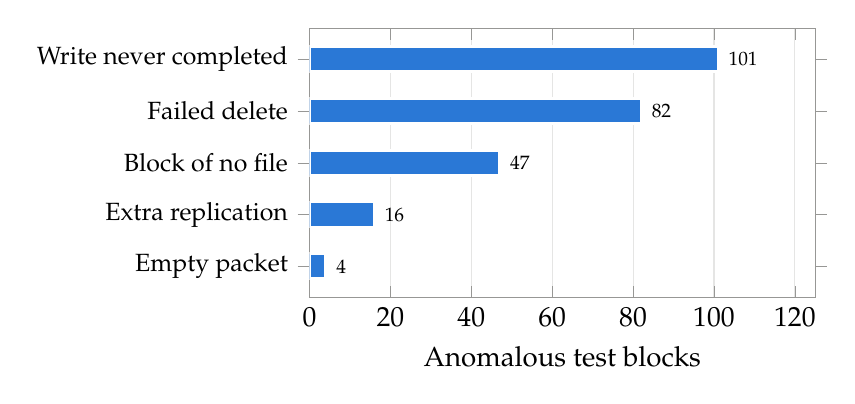
\begin{tikzpicture}
\begin{axis}[
  xbar, bar width=9pt, width=0.66\linewidth, height=5.0cm,
  xmin=0, xmax=125, xlabel={Anomalous test blocks},
  symbolic y coords={Empty packet, Extra replication, Block of no file, Failed delete, Write never completed},
  ytick=data, y tick label style={font=\small},
  nodes near coords, nodes near coords style={font=\scriptsize, text=black},
  xmajorgrids, grid style={inkmuted!15},
  axis line style={inkmuted!60}, tick style={inkmuted!60}, enlarge y limits=0.15]
\addplot[fill=seriesA, draw=white, line width=1pt] coordinates
  {(4,Empty packet) (16,Extra replication) (47,Block of no file) (82,Failed delete) (101,Write never completed)};
\end{axis}
\end{tikzpicture}
\caption{What is actually wrong with the 250 anomalous test blocks. The teacher mentions this
evidence in 1 explanation out of 250, the fine-tuned model in none.}
\label{fig:audit}
\end{figure}

Figure~\ref{fig:audit} shows the result. The evidence is always somewhere in the block, and
almost never in the line the model sees. Both models tell one of two stories, chosen by the
template of that line: an \code{allocateBlock} line becomes \emph{Erreur d'allocation de bloc}
(183 of 250 lines) and a \code{Receiving block} line becomes \emph{Connexion non autorisée}
(65 lines). Neither is supported by the logs: the allocation succeeded, and nothing in the
block points to an unauthorised connection. On normal lines the explanations are fine, since
they only describe the event. The fine-tuned model uses 8 distinct causes on the test set,
the teacher 19.

\subsection{End to end}
The pipeline was run on 3,000 consecutive blocks from the detection test period, with all
their lines (38,957 lines, 15 anomalous blocks). It flagged exactly the 15 anomalies, with no
false alarm, in 0.4 seconds. For 12 of them the missing events describe the failure: the block
was allocated and the transfer started, but \code{addStoredBlock} and \code{PacketResponder
terminating} never appear. For those 12 the line sent to the model is the \code{allocateBlock}
line, from which it can only guess. For the other 3, the selected line is the anomalous event
itself (a redundant \code{addStoredBlock}, an empty packet): line selection works when the
anomaly is something that happened, not when it is something that did not.

\subsection{Speed and cost}

\begin{table}[t]
\centering
\caption{Inference on a Tesla T4 (fp16, LoRA merged), 64 test lines, average request 161 tokens
in and 92 out. GPU at \$0.35 per hour; Groq at \$0.59 / \$0.79 per million input / output tokens.
The teacher cost is estimated from token counts of the same prompts and answers.}
\label{tab:cost}
\begin{tabular}{lrrrr}
\toprule
Setup & s / line & lines / s & tokens / s & USD / 1k lines \\
\midrule
Qwen2.5-1.5B + LoRA, batch 1 & 2.918 & 0.34 & 30 & 0.284 \\
Qwen2.5-1.5B + LoRA, batch 16 & 0.251 & 3.99 & 344 & \textbf{0.024} \\
Llama 3.3-70B on Groq (estimate) & & & & 0.168 \\
\bottomrule
\end{tabular}
\end{table}

One request at a time, the small model takes about 3 seconds per explanation and costs more
than the API, because the GPU is paid for while it waits (Table~\ref{tab:cost}). With batches
of 16 it is about 12 times faster and about 7 times cheaper than the teacher, with a peak GPU
memory of 3.4 GB. Running locally pays off only when explanations can be grouped, which is the
case when the detector flags many blocks at once. The GPU price covers the GPU alone, so the
real gap is somewhat smaller.

\section{Discussion}

\paragraph{The input decides what can be explained.} HDFS labels are per block and most
anomalies are visible only at the block level: an event that is absent, or a rare event in
another line. A model that sees one INFO line whose template also appears in normal blocks
has no information about the cause. The teacher did not have it either when it wrote the
training targets, so it guessed, and the student learned to reproduce the guess. Distillation
transfers whatever the teacher writes, hallucinations included, and metrics computed against
the teacher reward it for that.

\paragraph{Measuring against the teacher is not enough.} ROUGE-L and BERTScore against the
teacher rank the systems sensibly and show that fine-tuning works, yet they say nothing about
correctness. The audit, which only needs the raw logs and the detector's statistics, gives a
very different picture. Any evaluation of generated explanations needs at least one check
against the source data.

\paragraph{Cheap structure beats generation here.} The list of missing events comes for free
from the detector's training data and explains 40\% of the anomalous test blocks exactly; rare
events cover the rest. On HDFS, a structured description of the block is a better explanation
than a generated sentence about one line. A language model becomes useful again if its input
is that structured description, so that the cause can actually be read from it.

\paragraph{Detection is easy where templates are stable.} The logistic regression on template
counts is close to perfect on HDFS and loses to a one-line rule on BGL. The difference is the
template vocabulary, not the model.

\section{Limitations and future work}
\begin{itemize}
  \item There are no expert root causes for HDFS. The audit checks explanations against
        block-level evidence with keywords and a 50-example manual check, not against expert labels.
  \item The detector is supervised and needs complete sessions; PCA works without labels but its
        threshold does not carry over from one period to the next.
  \item The training data for the explanation model is small and repetitive: 69 anomalous lines,
        29 causes, 15 templates.
  \item Template extraction is a set of regular expressions designed for HDFS, which breaks down
        on BGL.
\end{itemize}
The next steps follow from the audit: give the model the whole flagged block, or the list of
missing and rare events, instead of a single line; re-annotate at the block level so that the
target cause is supported by the input; and replace the regular expressions with a learned
parser such as Drain so that detection holds on less regular systems.

\section{Conclusion}
A logistic regression on template counts detects HDFS anomalies almost perfectly, and a
1.5B-parameter model fine-tuned with LoRA reproduces the explanations of a 70B teacher better
than any baseline, at a fraction of the cost when requests are batched. But reproducing the
teacher is not the same as explaining the anomaly: neither model finds the evidence, because
it is not in the line they are given. Checking the explanations against the raw logs, rather
than against the teacher, is what revealed it.

\begin{thebibliography}{99}\small
\bibitem{xu2009} W.~Xu, L.~Huang, A.~Fox, D.~Patterson, M.~I.~Jordan.
  Detecting large-scale system problems by mining console logs. \emph{SOSP}, 2009.
\bibitem{he2016} S.~He, J.~Zhu, P.~He, M.~R.~Lyu.
  Experience report: system log analysis for anomaly detection. \emph{ISSRE}, 2016.
\bibitem{du2017} M.~Du, F.~Li, G.~Zheng, V.~Srikumar.
  DeepLog: anomaly detection and diagnosis from system logs through deep learning. \emph{CCS}, 2017.
\bibitem{zhu2023} J.~Zhu, S.~He, P.~He, J.~Liu, M.~R.~Lyu.
  Loghub: a large collection of system log datasets for AI-driven log analytics. \emph{ISSRE}, 2023.
\bibitem{oliner2007} A.~Oliner, J.~Stearley.
  What supercomputers say: a study of five system logs. \emph{DSN}, 2007.
\bibitem{he2017drain} P.~He, J.~Zhu, Z.~Zheng, M.~R.~Lyu.
  Drain: an online log parsing approach with fixed depth tree. \emph{ICWS}, 2017.
\bibitem{qwen2025} Qwen Team. Qwen2.5 technical report. arXiv:2412.15115, 2024.
\bibitem{hu2022} E.~J.~Hu, Y.~Shen, P.~Wallis, Z.~Allen-Zhu, Y.~Li, S.~Wang, L.~Wang, W.~Chen.
  LoRA: low-rank adaptation of large language models. \emph{ICLR}, 2022.
\bibitem{lin2004} C.-Y.~Lin. ROUGE: a package for automatic evaluation of summaries.
  \emph{ACL Workshop on Text Summarization Branches Out}, 2004.
\bibitem{zhang2020} T.~Zhang, V.~Kishore, F.~Wu, K.~Q.~Weinberger, Y.~Artzi.
  BERTScore: evaluating text generation with BERT. \emph{ICLR}, 2020.
\end{thebibliography}

\appendix
\section{Reproducing the results}
\begin{lstlisting}
python src/detect.py --log HDFS.log --labels anomaly_label.csv   # Table 1
python src/detect_bgl.py --log BGL.log                           # Table 2
python src/train.py                                              # LoRA training (GPU)
python src/evaluate.py                                           # Table 3 (GPU)
python src/audit_explanations.py --log HDFS.log                  # Figure 4
python src/pipeline.py --log HDFS_window_3k.log --top 10          # Section 4.5
python src/benchmark.py                                          # Table 4 (GPU)
python src/app.py --share                                        # live demo (GPU)
\end{lstlisting}

\section{Example}
A block whose write never completed (Loghub label: Anomaly). The pipeline output:
\begin{lstlisting}
blk_5679332564404011413   score 1.000   2 lines
missing: PacketResponder <N> for block <BLK> terminating
missing: Received block <BLK> of size <N> from /<IP>
missing: BLOCK* NameSystem.addStoredBlock: blockMap updated: <IP> is added to <BLK> size <N>
missing: Deleting block <BLK> file <PATH><BLK>
missing: BLOCK* NameSystem.delete: <BLK> is added to invalidSet of <IP>
line sent to the model:
081109 204403 35 INFO dfs.FSNamesystem: BLOCK* NameSystem.allocateBlock:
  /user/root/rand/_temporary/_task_200811092030_0001_m_000337_0/part-00337. blk_5679332564404011413
\end{lstlisting}
The fine-tuned model's answer for this kind of line:
\begin{lstlisting}
{"cause": "Erreur d'allocation de bloc",
 "raisonnement": "Étape 1 : Le système de fichiers HDFS tente d'allouer un bloc pour un fichier
 temporaire. Étape 2 : L'allocation du bloc échoue, ce qui indique une erreur dans le processus
 d'écriture de données. Étape 3 : ..."}
\end{lstlisting}
The allocation did not fail; the write that followed never completed.

\end{document}
